\section{Introduction}

With a long-anticipated migration of robots from factories to homes and offices, bridging
the gap between tasks defined in a high-level, natural language and plans
implemented on physical robots navigating a dynamic environment has become one
of the fundamental challenges in robotics.
% Most robots today are programmed in programming languages and end-user,
% specifically non-programmer, interaction is limited to a few simple settings.
%
Research in planning has focused on precise programming languages for robot tasks.
These languages are expressive, have a clear semantics,
and plans can be automatically generated~\cite{golog, strips, pddl,fainekosTemporalLogicMotionPlanning,hoffmanFF,ankushDrona}.
Unfortunately, the precision of such languages comes with unforgiving syntax.
Thus, it is hard for end-users to translate tasks in a natural language to valid programs.
The usual mechanism to incorporate natural language is to add a fixed set of ``syntactic sugar'' to express
commands in a structured subset \cite{hadasTranslatingStructuredEnglish}.
On the other hand, advances in natural language processing have enabled rich models of natural
language to be built, but the application to robot task planning is usually
limited to a fixed set of the most common scenarios~\cite{hadasProvablyCorrectReactiveControlFromNaturalLanguage,thomasonDialog,kollarDialog}.
Thus, users are either limited to a handful of natual language idioms,
or they can use their language freely, but the robot can only do a handful of actions.

In this paper, we present \tool, a system for end-users to program mobile robots using natural language.
The core of \tool is a high-level formal programming language for task specification.
A \emph{semantic parser} \cite{berantSempre} translates natural language utterances into internal representations for programs,
allowing more flexibility in specifying tasks.
While the core language is always available to programmers,
\tool further allows to extend the capability of the language and parsing through a
process of \emph{naturalization}~\cite{wangVoxelurn}.
Whenever the semantic parser fails to parse an utterance, the user can \emph{define} the
new utterance in terms of a sequence of utterances already understood (i.e., parseable) by the system.
The semantic parser generalizes the definition and adds it as a set of new production rules in the underlying language.
Thus, over time, \tool builds up a large lexicon of defined concepts through user interaction and generalization.
Initial users program in the core language, but build up idioms natural to the domain; future users
can use all concepts defined by the community previously.
Along the way, each parsed form retains the precise semantics of the core language.

Thus, \tool helps bridge the gap between expressive and precise programming languages with restricted syntax
and the flexible but ambiguous natural language.
While defined concepts are the usual way to express a formal language, for example using the library mechanism in a programming
language, \tool exploits two key features of the robotics domain.
First, it can provide quick visual feedback to the user about the \emph{effect} of an utterance by simulating
the plan on the world.
This allows quick resolution of ambiguity.
Second, unlike a library in a general purpose language, in which a programmer parameterizes a function explicitly,
\tool uses grammar induction within the parser to generalize from concrete utterances.
While grammar induction may not be powerful enough for general-purpose computation, it works remarkably well
in the restricted context of planning worlds.


\begin{figure}[t]
\resizebox{\linewidth}{!}{
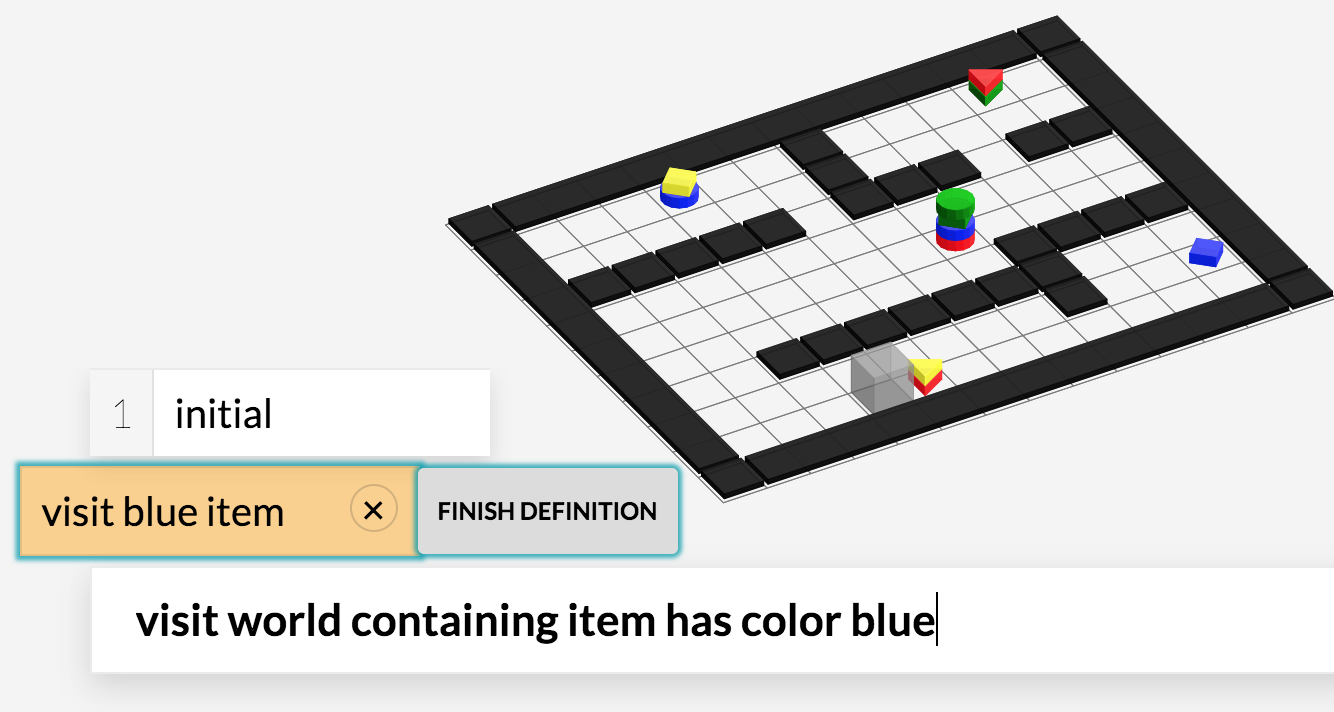
\includegraphics{images/flipperSimplestSimulation.png}
}
\caption{Simulation world of \tool}
\label{fig:simulationWorld}
\end{figure}


\smallskip
\noindent
\textbf{Interacting with \tool}
Let us be more specific.
The user of \tool instructs a single robot which moves in a world
consisting of several connected rooms separated by walls, presenting obstacles for the robot.
These rooms contain a number of items with different properties; for simplicity we consider here different
colors and shapes.
The robot can modify this world by moving to free locations,
and by applying a set of actions, such as picking up or dropping items.
Figure~\ref{fig:simulationWorld} shows a simulation of such a world.
The user specifies actions for the robot as an utterance.
For example, the utterance (in the core language) \lstinline{visit world containing item has color blue}
instructs the robot to visit some point that contains a blue item.
\tool parses the utterance into a task specification in the core language, constructs a plan over the simulated
world, and provides visual feedback first, showing what the robot would do.
This is especially useful if there are multiple possible interpretations, e.g., due to ambiguities
in the semantic parsing.
Once the user selects an interpretation, the robot proceeds with an action (ideally,
in the real world; in our current implementation, still in simulation). 

In case the plan is unrealizable, the user receives feedback specifying which primitive part of the
action is not realizable.

It is possible, however, that \tool is not able to parse a command.
For example, the user might state ``visit blue item'' to specify the same task in a more natural way.
In this case, \tool asks the user to define this utterance
in terms of one or more parseable commands already understood by the system.
This is the situation in Figure \ref{fig:simulationWorld}.
\tool generalizes the definition and creates new grammar rules.
Thus, it can now also understand the utterance ``visit red item.''


We have implemented \tool on top of Sempre~\cite{berantSempre}, the trainable semantic parser, its interactive version introduced by the Voxelurn
naturalization tool \cite{wangVoxelurn}, and a temporal path planner.
In a preliminary study on thirteen users (with programming experience), we demonstrate that naturalization
helps specify tasks in a more succinct way, that users define derived concepts as building blocks,
and these derived concepts are reused by later users as their basis for interacting with the system.


% The architecture of \tool has four main components. The first is a formal core language to express temporal objectives in the world (described in the Section \ref{sec:coreLanguage}). The second is an adaptive language component consisting of a semantic parser and a grammar inducer. The role of the semantic parser is to map natural language utterances into their meaning, assign each of them a score according to the model and update the model based on user's choices. Grammar inducer creates new rules from the definitions provided by the user. The adaptive language component is described in the Section \ref{sec:naturalization}.
% The third is a planner that, given a logical representation of a goal, generates a plan for the robot to execute it goal if possible. Finally, a visual user interface provides the user real-time feedback by exhibiting the effect of a plan in a simulated environment.

